%!TEX root = ../../book_ML.tex
\chapter{Lọc cộng tác phân tích ma trận}
% \chapter{Matrix factorization collaborative filtering}
\label{cha:matrix_factorization}
% \index{matrix factorization: phân tích ma trận thành nhân tử}
\section{Giới thiệu }
Trong Chương~\ref{cha:CF}, chúng ta đã làm quen với phương pháp
lọc cộng tác dựa trên hành vi của người dùng hoặc sản phẩm lân cận. Trong chương này, chúng ta sẽ làm quen với một hướng
tiếp cận khác cho lọc cộng tác dựa trên bài toán
\textit{phân tích ma trận thành nhân tử} ({matrix factorization} hoặc
{matrix decomposition}). Phương pháp này được gọi
là \textit{lọc cộng tác phân tích ma trận} ({matrix factorization collaborative filtering} -- MFCF)~\cite{koren2009matrix}.

Nhắc lại rằng trong hệ thống gợi ý dựa trên nội dung, mỗi sản phẩm được
mô tả bằng một vector thông tin $\bx$. Trong phương pháp
đó, ta cần tìm một vector trọng số $\bw$ tương ứng với mỗi người dùng sao cho các đánh giá đã biết của người dùng tới các sản phẩm được xấp xỉ bởi:
\begin{equation} 
y \approx \bx^T\bw
\end{equation} 
Với cách làm này, ma trận tiện ích $\mathbf{Y}$, \textit{giả sử đã được điền
hết}, sẽ xấp xỉ với:
\begin{equation} 
    \mathbf{Y} \approx \left[ \begin{matrix} \bx^T_1\bw_1 &
    \bx^T_1\bw_2 & \dots & \bx^T_1 \bw_N\\\
    \bx^T_2\bw_1 & \bx^T_2\bw_2 & \dots &
    \bx^T_2 \bw_N\\\ \dots & \dots & \ddots & \dots \\\
    \bx^T_M\bw_1 & \bx^T_M\bw_2 & \dots & \bx^T_M \bw_N \end{matrix} \right] = \left[ \begin{matrix} \bx^T_1 \\\ \bx^T_2 \\\ \dots \\\ \bx^T_M  \end{matrix} \right] 
    \left[ \begin{matrix} \bw_1 & \bw_2 & \dots & \bw_N \end{matrix} \right] = \bX^T\bW 
\end{equation} 
với $M, N$ lần lượt là số lượng sản phẩm và người dùng. Chú ý rằng trong
hệ thống gợi ý dựa trên nội dung, $\bx$ được xây dựng dựa trên thông
tin mô tả của sản phẩm và quá trình xây dựng này độc lập với quá trình đi
tìm hệ số phù hợp cho mỗi người dùng. Như vậy, việc xây dựng thông tin sản phẩm đóng vai trò quan trọng và có ảnh hưởng trực tiếp tới hiệu năng của
mô hình. Thêm nữa, việc xây dựng từng mô hình riêng lẻ cho mỗi người dùng dẫn
đến kết quả chưa thực sự tốt vì không khai thác được mối quan hệ giữa
người dùng.
 
Bây giờ, giả sử rằng không cần xây dựng trước thông tin sản phẩm
$\bx$ mà vector này có thể được huấn luyện đồng thời với mô hình của mỗi người dùng (ở đây là một vector trọng số). Điều này nghĩa là, biến số trong bài toán tối ưu là cả
$\bX$ và $\bW$; trong đó,
mỗi cột của $\bX$ là thông tin về một sản phẩm, mỗi cột của $\bW$ là mô hình của một người dùng. 

 
Với cách làm này, chúng ta đang cố gắng xấp xỉ ma trận tiện ích $\mathbf{Y} \in
\mathbb{R}^{M \times N}$ bằng tích của hai ma trận $\bX\in
\mathbb{R}^{K\times M}$ và $\bW \in \mathbb{R}^{K \times N}$. Thông
thường, $K$ được chọn là một số nhỏ hơn so với $M, N$. Khi đó, cả hai
ma trận $\bX$ và $\bW$ đều có hạng không vượt quá $K$. Chính vì
vậy, phương pháp này còn được gọi là \textit{phân tích ma trận hạng thấp} ({low-rank matrix factorization}) (xem
Hình~\ref{fig:25_1}).
% ******************************************************************************
\begin{figure}[t]
\centering
    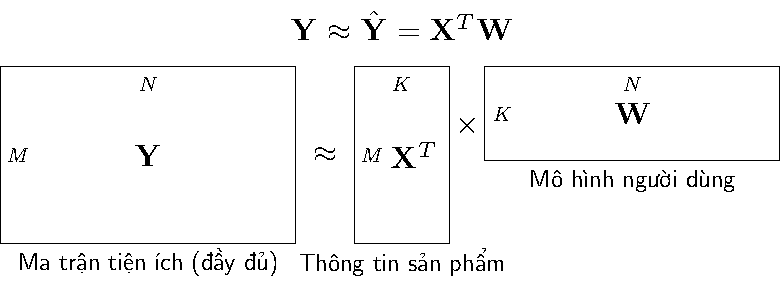
\includegraphics[width = .7\textwidth]{Chapters/06_RecommendationSystems/25_mf/latex/mf1.pdf}
    \caption[]{Phân tích ma trận. Ma trận tiện ích $\mathbf{Y} \in
    \R^{M\times N}$ được
    xấp xỉ bởi tích của hai ma trận $\bX \in \R^{M\times K}$ và
    $\bW \in \R^{K\times N}$.}
    \label{fig:25_1}
\end{figure}
% ******************************************************************************
 
Một vài điểm cần lưu ý:  
\begin{itemize}
    \item Ý tưởng chính đằng sau lọc cộng tác phân tích ma trận
    là tồn tại các \textit{đặc trưng ẩn} ({latent feature}) mô tả mối quan hệ
    giữa sản phẩm và người dùng. Ví dụ, trong hệ thống khuyến nghị các bộ phim,
    đặc trưng ẩn có thể là \textit{hình sự}, \textit{chính trị}, \textit{hành
    động}, \textit{hài},...; cũng có thể là một sự kết hợp nào đó của các thể
    loại này. Đặc trưng ẩn cũng có thể là bất cứ điều gì mà chúng ta không thực
    sự cần đặt tên. Mỗi sản phẩm sẽ mang đặc trưng ẩn ở một mức độ nào đó tương
    ứng với các hệ số trong vector $\bx$ của nó, hệ số càng cao tương ứng với
    việc mang tính chất đó càng cao. Tương tự, mỗi người dùng cũng sẽ có xu
    hướng thích những tính chất ẩn nào đó được mô tả bởi các hệ số trong
    vector $\bw$. Hệ số cao tương ứng với việc người dùng thích các bộ phim có
    tính chất ẩn đó nhiều. Giá trị của biểu thức $\bx^T\bw$ sẽ cao nếu các thành phần
    tương ứng của $\bx$ và $\bw$ đều cao (và dương) hoặc đều thấp (và âm). Điều này nghĩa là sản phẩm
    mang các tính chất ẩn mà người dùng thích, vậy ta nên gợi ý sản phẩm này cho
    người dùng đó.
     
    \item Tại sao phân tích ma trận được xếp vào lọc cộng tác?
    Câu trả lời đến từ việc tối ưu hàm mất mát được thảo luận ở
    Mục~\ref{sec:2_2}. Về cơ bản, để tìm nghiệm của bài toán tối ưu, ta phải lần
    lượt đi tìm $\bX$ và $\bW$ khi thành phần còn lại được cố
    định. Như vậy, mỗi cột của $\bX$ sẽ phụ thuộc vào toàn bộ các cột
    của $\bW$. Ngược lại, mỗi cột của $\bW$ phụ thuộc vào
    toàn bộ các cột của $\bX$. Như vậy, có những mỗi quan hệ ràng buộc
    {chằng chịt} giữa các thành phần của hai ma trận trên. Vì vậy, phương pháp này
    cũng được xếp vào lọc cộng tác. 
     
    \item Trong các bài toán thực tế, số lượng sản phẩm $M$ và số lượng
    người dùng $N$ thường rất lớn. Việc tìm ra các mô hình đơn giản giúp dự
    đoán độ quan tâm cần được thực hiện một cách nhanh nhất có thể.
    Lọc cộng tác dựa trên lân cận không yêu cầu việc huấn luyện quá
    nhiều, nhưng trong quá trình dự đoán, ta cần đi tìm độ tương tự của một người dùng với toàn bộ
    người dùng còn lại rồi suy ra kết quả. Ngược lại, với phân tích ma trận, việc huấn luyện tạp hơn vì phải
    lặp đi lặp lại việc tối ưu một ma trận khi cố định ma trận còn lại. Tuy nhiên,
    việc dự đoán đơn giản hơn vì chỉ cần tính tích vô hướng
    $\bx^T\bw$, mỗi vector có độ dài $K$ là một số nhỏ hơn nhiều so với
    $M, N$. Vì vậy, quá trình dự đoán không yêu cầu nặng về tính toán. Việc này khiến phân tích ma trận trở nên phù hợp với các mô hình có tập dữ liệu lớn.
     
    \item Hơn nữa, việc lưu trữ hai ma trận $\bX$ và $\bW$ yêu
    cầu lượng bộ nhớ nhỏ so với việc lưu toàn bộ ma trận tiện ích và 
    tương tự trong lọc cộng tác lân cận. Cụ thể, ta cần
    bộ nhớ để chứa $K(M+N)$ phần tử thay vì $M^2$ hoặc $N^2$ của ma trận
    tương tự ($K \ll M, N$).  
\end{itemize}
 
 
 
\section{Xây dựng và tối ưu hàm mất mát}
\label{sec:2_2}
\subsection{Xấp xỉ các đánh giá đã biết}
Như đã đề cập, đánh giá của người dùng $n$ tới sản phẩm $m$ có thể được xấp xỉ
bởi $y_{mn} = \bx^T_m\bw_n$. Ta cũng có thể thêm các hệ số điều chỉnh vào công thức xấp xỉ
này và tối ưu các hệ số đó. Cụ thể: 
\begin{equation}
    y_{mn} \approx \bx_m^T \bw_n + b_m + d_n
\end{equation}
Trong đó, $b_m$ và $d_n$ lượt lượt là các hệ số điều chỉnh ứng với sản phẩm
$m$ và người dùng $n$. Vector $\bb = [b_1, b_2, \dots, b_M]^T$ là vector điều chỉnh
cho các sản phẩm, vector $\bd = [d_1, d_2, \dots, d_N]^T$ là vector điều chỉnh cho các
người dùng. Giống như lọc cộng tác lân cận (NBCF),
các giá trị này cũng có thể được coi là các giá trị giúp chuẩn hoá dữ liệu với
$\bb$ tương ứng với lọc cộng tác sản phẩm và $\bd$ tương ứng với lọc cộng tác người dùng. Không
giống như trong NBCF, các vector này sẽ được tối ưu để tìm ra các giá trị phù hợp với tập huấn luyện nhất. Thêm vào đó, huấn luyện $\bd$ và
$\bb$ cùng lúc giúp kết hợp cả lọc cộng tác người dùng và lân cận vào một bài toán tối
ưu. Vì vậy, chúng ta mong đợi rằng phương pháp này sẽ mang lại hiệu quả tốt hơn.


\subsection{Hàm mất mát }
% Tương tự như trong content-based recommendation system, hàm mất
% mát của matrix factorization collaborative filtering cũng được xây dựng dựa
% trên các thành phần đã được điền của ma trận utility $\mathbf{Y}$, có
% khác một chút là không có thành phần bias và biến tối ưu là cả $\bX$ và $\bW$. Việc thêm bias vào sẽ được thảo luận ở Mục. Việc xây dựng hàm mất mát cho Matrix Factorization là tương đối dễ hiểu:

Hàm mất mát cho MFCF có thể được viết như sau: 
\begin{equation*}
    \mathcal{L}(\bX, \bW, \bb, \bd) = \underbrace{\frac{1}{2s}\sum_{n=1}^N
    \sum_{m:r_{mn} =
        1} (\bx_m^T\bw_n + b_m + d_n - y_{mn})^2}_{\text{mất mát trên dữ liệu}} +
        \underbrace{\frac{\lambda}{2}(\|\bX\|_F^2 +
            \|\bW\|_F^2)}_{\text{mất mát kiểm soát}}
\end{equation*}
trong đó $r_{mn} = 1$ nếu sản phẩm thứ $m$ đã được đánh giá bởi người dùng thứ
$n$, $s$ là số lượng đánh giá đã biết trong tập huấn luyện, $y_{mn}$ là đánh giá chưa chuẩn hoá\footnote{việc chuẩn hoá sẽ được tự động thực hiện
thông qua việc huấn luyện $\bb$ và $\bd$} của người dùng thứ $n$ tới sản phẩm
thứ $m$. Thành phần thứ nhất của hàm mất mát chính là sai số trung
bình bình phương sai số của mô hình. Thành phần thứ hai chính là kiểm soát 
$l_2$ giúp mô hình tránh quá khớp. 
% \textbf{Lưu ý:} Giá trị \textit{ratings} thường là các giá trị đã được chuẩn hoá, bằng cách trừ mỗi hàng của Utility Matrix đi trung bình cộng của các giá trị đã biết của hàng đó (item-based) hoặc trừ mỗi cột đi trung bình cộng của các giá trị đã biết trong cột đó (user-based). Trong một số trường hợp nhất định, ta không cần chuẩn hoá ma trận này, nhưng kèm theo đó phải có thêm các kỹ thuật khác để giải quyết vấn đề \textit{thiên lệch} trong khi \textit{rating}. 
 
Việc tối ưu đồng thời $\bX, \bW, \bb, \bd$ là tương đối phức tạp. Phương pháp được sử dụng là lần lượt tối ưu một trong hai cặp
$(\bX, \bb)$, $(\bW, \bd)$ trong lúc cố định cặp còn lại. Quá trình này được lặp
đi lặp lại cho tới khi hàm mất mát hội tụ.
 
\subsection{Tối ưu hàm mất mát }
Khi cố định cặp $(\bX, \bb)$, bài toán tối ưu cặp $(\bW, \bd)$ có thể được tách
thành $N$ bài toán nhỏ:
\begin{equation} 
\label{eqn:25_2}
\mathcal{L}_1(\bw_n, d_n) = \frac{1}{2s} \sum_{m:r_{mn} = 1}
(\bx_m^T\mathbf{w}_n + b_m + d_n - y_{mn})^2 + \frac{\lambda}{2}
\|\mathbf{w_n}\|_F^2
\end{equation} 
Mỗi bài toán có thể được tối ưu bằng gradient descent. Công việc quan trọng là tính các gradient của từng hàm mất mát nhỏ này theo $\bw_n$ và
$d_n$.
 Vì biểu thức trong dấu $\sum$ chỉ phụ thuộc vào các sản phẩm đã được đánh
giá bởi người dùng thứ $n$ (tương ứng với các $r_{mn}  = 1$), ta có thể đơn
giản~\eqref{eqn:25_2} bằng cách đặt $\hat{\bX}_n$ là ma trận con được tạo bởi
các cột của $\bX$ tương ứng với các sản phẩm đã được đánh giá bởi
người dùng $n$, $\hat{\bb}_n$ là vector điều chỉnh con tương ứng, và
$\hat{\mathbf{y}}_n$ là các đánh giá tương ứng. Khi đó,
\begin{equation} 
\mathcal{L}_1(\mathbf{w}_n, d_n) = \frac{1}{2s} \|\hat{\bX}^T_n\bw_n +
\hat{\bb}_n
+ d_n\bone - \hat{\by}_n\|^2 + \frac{\lambda}{2}\|\bw_n\|_2^2
\end{equation} 
với $\bone$ là vector với mọi phần tử bằng một với kích thước phù hợp. Các gradient 
của nó là:
\begin{eqnarray} 
% \frac{\partial \mathcal{L}_1}{\partial \bw_n} 
\nabla_{\bw_n}\mathcal{L}_1
&=&
\frac{1}{s}\hat{\bX}_n(\hat{\bX}_n^T\bw_n + \hat{\bb}_n + d_n\bone -
\hat{\by}_n) + \lambda \bw_n \\\
% \frac{\partial \mathcal{L}_1}{\partial d_n} 
\nabla_{b_n}\mathcal{L}_1
&=&
\frac{1}{s}\bone^T(\hat{\bX}_n^T\bw_n + \hat{\bb}_n + d_n\bone -
\hat{\by}_n)
\end{eqnarray} 
\bi{Công thức cập nhật cho $\bw_n$ và $d_n$:}
% \vspace{-.5cm}
\begin{eqnarray} 
\bw_n &\assign& \bw_n - \eta \left(\frac{1}{s}\hat{\bX}_n(\hat{\bX}_n^T\bw_n +
\hat{\bb}_n + d_n\bone - \hat{\by}_n) + \lambda \bw_n\right) \\
d_n &\assign& d_n - \eta \left(\frac{1}{s}\bone^T(\hat{\bX}_n^T\bw_n + \hat{\bb}_n + d_n\bone -
\hat{\by}_n)\right)
\end{eqnarray} 
Tương tự, mỗi cột $\bx_m$ của $\bX$ và $b_m$ sẽ được tìm bằng cách tối ưu bài toán 
\begin{eqnarray} 
\label{eqn:25_xm}
\mathcal{L}_2(\bx_m, b_m) &=& \frac{1}{2s}\sum_{n:r_{mn} = 1}
(\bw_n^T\bx_m + d_n  + b_m - y_{mn})^2 + \frac{\lambda}{2}\|\bx_m\|_2^2
\end{eqnarray}
Đặt $\hat{\bW}_m$ là ma trận con tạo bởi các cột của $\bW$ ứng
với các người dùng đã đánh giá sản phẩm $m$, $\hat{\bd}_m$ là vector điều chỉnh con
tương ứng, và $\hat{\mathbf{y}}^m$ là vector các đánh giá tương ứng. Bài
toán~\eqref{eqn:25_xm} trở thành
\begin{equation} 
\mathcal{L}(\bx_m, b_m) 
 = \frac{1}{2s}\|\hat{\bW}_m^T\bx_m + \hat{\bd}_m + b_n\bone - \hat{\by}_m \| +
 \frac{\lambda}{2}\|\bx_m\|_2^2.
 % \hat{\mathbf{y}}^m - {\bx}_m\hat{\bW}_m\|_2^2 + \frac{\lambda}{2} \|\bx_m\|_2^2
\end{equation} 
Tương tự ta có  

\bi{Công thức cập nhật cho $\bx_m$ và $b_m$:}
% \vspace{-.5cm}
\begin{eqnarray}
    \bx_m &\assign & \bx_m -
    \eta\left(\frac{1}{s}\hat{\bW}_m(\hat{\bW}_m^T\bx_m + \hat{\bd}_m +
    b_n\bone - \hat{\by}_m) + \lambda\bx_m\right) \\
    b_m &\assign& b_m - \eta\left(\frac{1}{s}\bone^T(\hat{\bW}_m^T\bx_m + \hat{\bd}_m +
    b_n\bone - \hat{\by}_m)\right)
\end{eqnarray} 

% Trong mục tiếp theo, chúng ta sẽ giải quyết bài toán này trên Python. 
\section{Lập trình Python }
Chúng ta sẽ viết một \pythoninline{class MF} thực hiện việc tối ưu
các biến với ma trận tiện ích được cho dưới dạng \pythoninline{Y_data} giống
như với NBCF. 

Trước tiên, ta khai báo một vài thư viện cần thiết và khởi tạo
\pythoninline{class MF}:
\begin{lstlisting}[language=Python]
from __future__ import print_function 
import pandas as pd 
import numpy as np
from sklearn.metrics.pairwise import cosine_similarity
from scipy import sparse 

class MF(object):
    def __init__(self, Y, K, lam = 0.1, Xinit = None, Winit = None, 
                 learning_rate = 0.5, max_iter = 1000, print_every = 100):
        self.Y      = Y    # represents the utility matrix 
        self.K      = K    # 
        self.lam    = lam  # regularization parameter 
        self.learning_rate = learning_rate # for gradient descent 
        self.max_iter      = max_iter # maximum number of iterations 
        self.print_every   = print_every # print loss after each a few iters 
        self.n_users       = int(np.max(Y[:, 0])) + 1 
        self.n_items       = int(np.max(Y[:, 1])) + 1
        self.n_ratings     = Y.shape[0] # number of known ratings
        self.X =\ 
            np.random.randn(self.n_items, K) if Xinit is None else Xinit 
        self.W =\ 
            np.random.randn(K, self.n_users) if Winit is None else Winit 
        self.b = np.random.randn(self.n_items) # item biases
        self.d = np.random.randn(self.n_users) # user biases
\end{lstlisting} 
Tiếp theo, chúng ta viết các phương thức
\pythoninline{loss, updateXb, updateWd} cho \pythoninline{class MF}. 
% \newpage 
\begin{lstlisting}[language=Python]
    def loss(self):
        L = 0 
        for i in range(self.n_ratings):
            # user_id, item_id, rating
            n, m, rating = int(self.Y[i,0]), int(self.Y[i,1]), self.Y[i,2]
            L += 0.5*(self.X[m].dot(self.W[:, n])\ 
                + self.b[m] + self.d[n] - rating)**2    
        
        L /= self.n_ratings
        # regularization, don't ever forget this 
        return L + 0.5*self.lam*(np.sum(self.X**2) + np.sum(self.W**2))

    def updateXb(self):
        for m in range(self.n_items):
            # get all users who rated item m and corresponding ratings
            ids = np.where(self.Y[:, 1] == m)[0] # row indices of items m 
            user_ids,ratings=self.Y[ids, 0].astype(np.int32),self.Y[ids, 2]
            Wm, dm = self.W[:, user_ids], self.d[user_ids]
            for i in range(30): # 30 iteration for each sub problem 
                xm = self.X[m]
                error = xm.dot(Wm) + self.b[m] + dm  - ratings 
                grad_xm = error.dot(Wm.T)/self.n_ratings + self.lam*xm
                grad_bm = np.sum(error)/self.n_ratings
                # gradient descent
                self.X[m] -= self.learning_rate*grad_xm.reshape(-1)
                self.b[m] -= self.learning_rate*grad_bm
    
    def updateWd(self): # and d 
        for n in range(self.n_users):
            # get all items rated by user n, and the corresponding ratings
            ids = np.where(self.Y[:,0] == n)[0] #indexes of items rated by n 
            item_ids,ratings=self.Y[ids, 1].astype(np.int32), self.Y[ids, 2]
            Xn, bn = self.X[item_ids], self.b[item_ids]
            for i in range(30): # 30 iteration for each sub problem 
                wn = self.W[:, n]
                error = Xn.dot(wn) + bn + self.d[n] - ratings
                grad_wn = Xn.T.dot(error)/self.n_ratings + self.lam*wn
                grad_dn = np.sum(error)/self.n_ratings
                # gradient descent
                self.W[:, n] -= self.learning_rate*grad_wn.reshape(-1)
                self.d[n]    -= self.learning_rate*grad_dn
\end{lstlisting} 
% \index{RMSE}
Phần tiếp theo là quá trình tối ưu chính của MF (\pythoninline{fit}), dự đoán
đánh giá (\pythoninline{pred}) và
đánh giá chất lượng mô hình bằng RMSE (\pythoninline{evaluate_RMSE}). 
\begin{lstlisting}[language=Python]
    def fit(self):
        for it in range(self.max_iter):
            self.updateWd()
            self.updateXb()
            if (it + 1) % self.print_every == 0:
                rmse_train = self.evaluate_RMSE(self.Y)
                print('iter = %d, loss = %.4f, RMSE train = %.4f'%(it + 1, 
                    self.loss(), rmse_train))
\end{lstlisting} 
% \newpage 
\begin{lstlisting}[language=Python]
    def pred(self, u, i):
        """ 
        predict the rating of user u for item i 
        """
        u, i = int(u), int(i)
        pred = self.X[i, :].dot(self.W[:, u]) + self.b[i] + self.d[u]
        return max(0, min(5, pred)) # 5-scale in MoviesLen 
    
    def evaluate_RMSE(self, rate_test):
        n_tests = rate_test.shape[0] # number of test 
        SE = 0 # squared error
        for n in range(n_tests):
            pred = self.pred(rate_test[n, 0], rate_test[n, 1])
            SE += (pred - rate_test[n, 2])**2 

        RMSE = np.sqrt(SE/n_tests)
        return RMSE
\end{lstlisting}

Tới đây, class \pythoninline{MF} đã được xây dựng với các phương thúc 
cần thiết. Ta cần kiểm tra chất lượng mô hình khi áp dụng
lên tập dữ liệu MoviesLen 100k:
\begin{lstlisting}[language=Python]
r_cols = ['user_id', 'movie_id', 'rating', 'unix_timestamp']
ratings_base = pd.read_csv('ml-100k/ua.base', sep='\t', names=r_cols)
ratings_test = pd.read_csv('ml-100k/ua.test', sep='\t', names=r_cols)

rate_train = ratings_base.as_matrix()
rate_test = ratings_test.as_matrix()

# indices start from 0
rate_train[:, :2] -= 1
rate_test[:, :2] -= 1

rs = MF(rate_train, K = 50, lam = .01, print_every = 5, learning_rate = 50, 
        max_iter = 30)
rs.fit()
# evaluate on test data
RMSE = rs.evaluate_RMSE(rate_test)
print('\nMatrix Factorization CF, RMSE = %.4f' %RMSE)
\end{lstlisting}
\kq 
\begin{lstlisting}
iter = 5, loss = 0.4447, RMSE train = 0.9429
iter = 10, loss = 0.4215, RMSE train = 0.9180
iter = 15, loss = 0.4174, RMSE train = 0.9135
iter = 20, loss = 0.4161, RMSE train = 0.9120
iter = 25, loss = 0.4155, RMSE train = 0.9114
iter = 30, loss = 0.4152, RMSE train = 0.9110

Matrix Factorization CF, RMSE = 0.9621
\end{lstlisting}

RMSE thu được là 0.9621, tốt hơn so với NBCF trong chương trước (0.9688). 

\section{Thảo luận}
\label{sec:25_4}
 
% \subsection{Khi có bias}
% Một lợi thế của hướng tiếp cận Matrix Factorization cho Collaborative Filtering là khả năng linh hoạt của nó khi có thêm các điều kiện ràng buộc khác, các điều kiện này có thể liên quan đến quá trình xử lý dữ liệu hoặc đến từng ứng dụng cụ thể.  
 
% Giả sử ta chưa chuẩn hoá các giá trị \textit{ratings} mà sử dụng trực tiếp giá trị ban đầu của chúng trong đẳng thức $(1)$. Việc chuẩn hoá cũng có thể được tích hợp trực tiếp vào trong hàm mất mát. Như tôi đã đề cập, các \textit{ratings} thực tế đều có những thiên lệch về người dùng hoặc/và sản phẩm. Có người dùng dễ và khó tính, cũng có những sản phẩm được \textit{rated} cao hơn những sản phẩm khác chỉ vì người dùng thấy các người dùng khác đã đánh giá sản phẩm đó cao rồi. Vấn đề thiên lệch có thể được giải quyết bằng các biến gọi là \textit{biases}, phụ thuộc vào mỗi người dùng và sản phẩm và có thể được tối ưu cùng với $\bX$ và $\bW$. Khi đó, \textit{ratings} của người dùng $n$ lên sản phẩm $m$ không chỉ được xấp xỉ bằng $\bx_m\bw_n$ mà còn phụ thuộc vào các \textit{biases} của sản phẩm $m$ và người dùng $n$ nữa. Ngoài ra, giá trị này cũng có thể phụ thuộc vào giá trị trung bình của toàn bộ \textit{ratings} nữa:  
 
% \begin{equation} 
% y_{mn} \approx \bx_m \bw_n + b_m + d_n + \mu 
% \end{equation} 
 
% với $b_m, d_n, \mu$ lần lượt là bias của sản phẩm $m$, người dùng $n$, và giá trị trung bình của toàn bộ các \textit{ratings} (là hằng số).  
 
% Lúc này, hàm mất mát có thể được thay đổi thành:   
% \begin{eqnarray} 
% \mathcal{L}(\bX, \bW, \mathbf{b}, \mathbf{d}) &=& \frac{1}{2s} \sum_{n=1}^N \sum_{m:r_{mn} = 1} (\bx_m\bw_n + b_m + d_n +\mu - y_{mn})^2 + \\\  
% && + \frac{\lambda}{2} (\|\bX\|_F^2 + \|\bW\|_F^2 + \|\mathbf{b}\|_2^2  + \|\mathbf{d}\|_2^2) 
% \end{eqnarray}  
 
% Việc tính toán đạo hàm cho từng biến không quá phức tạp, tôi sẽ không bàn tiếp ở đây. Tuy nhiên, nếu bạn quan tâm, bạn có thể tham khảo \href{https://github.com/tiepvupsu/tiepvupsu.github.io/tree/master/assets/25_mf/python}{source code mà tôi viết tại đây}. Link này cũng kèm theo các ví dụ nêu trong Mục 3 và dữ liệu liên quan.  
 
\index{phân tích ma trận không âm -- nonnegative matrix factorization, NMF}
\index{NMF}
\begin{itemize}
    \item \textbf{Phân tích ma trận không âm:}. Khi ma trận tiện ích chưa được
    chuẩn hoá, các phần tử đều là giá trị không âm. Kể cả trong trường hợp dải
    giá trị của các đánh giá có chứa giá trị âm, ta chỉ cần cộng thêm vào ma
    trận tiện ích một giá trị hợp lý để có được các thành phần là các số
    không âm. Khi đó, một phương pháp phân tích ma trận thường mang lại hiệu quả cao trong các hệ thống gợi ý là \textit{phân tích ma trận không âm} ({nonnegative matrix factorization} -- NMF)~\cite{zhang2006learning}, tức phân tích ma trận thành tích các ma
    trận có các phần tử không âm. Lúc này, đặc trưng ẩn của một sản phẩm và hệ số tương ứng của người dùng là các số không âm. 
    % Nếu sản phẩm không có đặc trưng ẩn này, thành phần tương ứng của $\bx$ sẽ bằng không thay vì âm. Việc này một người dùng có khả năng thích sản phẩm này hay không không phụ thuộc vào đặc trưng này. 
 
    Thông qua phân tích ma trận, người dùng và sản phẩm được liên
    kết với nhau bởi các \textit{đặc trưng ẩn}. Độ liên kết của mỗi
    người dùng và sản phẩm tới mỗi đặc trưng ẩn được đo bằng thành phần tương
    ứng trong vector đặc trưng, giá trị càng lớn thể hiện việc
    người dùng hoặc sản phẩm có liên quan đến đặc trưng ẩn đó càng lớn.
    Bằng trực giác, sự liên quan của một người dùng hoặc sản phẩm đến
    một đặc trưng ẩn nên là một số không âm với giá trị không thể hiện việc không liên quan thay vì giá trị âm. Hơn nữa, mỗi người dùng và sản phẩm chỉ liên quan đến một vài đặc trưng ẩn nhất định. Vì vậy, các vector
    đặc trưng cho người dùng và sản phẩm nên là các vector không âm và
    có rất nhiều giá trị bằng không. Những nghiệm này có thể đạt được bằng cách cho
    thêm ràng buộc không âm vào các thành phần của $\bX$ và $\bW$. Đây
    chính là nguồn gốc của ý tưởng và tên gọi phân tích ma trận không âm.
 
 \index{phân tích ma trận điều chỉnh nhỏ -- incremental matrix factorization}

    \item \textbf{Phân tích ma trận điều chỉnh nhỏ}: thời gian dự
    đoán của một hệ thống gợi ý sử dụng phân tích ma trận là rất nhanh nhưng
    thời gian huấn luyện là khá lâu với các bài toán quy mô lớn. Thực tế cho thấy,
    ma trận tiện ích thay đổi liên tục vì có thêm người dùng, sản phẩm cũng như
    các đánh giá mới, vì vậy các tham số mô hình cũng phải thường xuyên được cập
    nhật. Điều này đồng nghĩa với việc ta phải tiếp tục thực hiện quá trình huấn
    luyện vốn tốn khá nhiều thời gian. Thay vì huấn luyện lại toàn bộ mô hình,
    ta có thể điều chỉnh các ma trận $\bX$ và $\bW$ bằng cách huấn luyện thêm
    một vài vòng lặp. Kỹ thuật này được gọi là \textit{phân tích ma trận điều
    chỉnh nhỏ} ({incremental matrix factorization})~\cite{vinagre2014fast}, được
    áp dụng nhiều trong các bài toán quy mô lớn.
 
 
    \item Có nhiều các giải bài toán tối ưu của phân tích ma trận ngoài cách áp dụng gradient descent. Bạn đọc có thể xem thêm
    \textit{alternating least square (ALS)} (\url{https://goo.gl/g2M4fb}),
    \textit{generalized low rank models} (\url{https://goo.gl/DrDWyW}), và
    \textit{phân tích giá trị suy biến}~\cite{sarwar2002incremental,paterek2007improving}.
    Chương~\ref{cha:svd} sẽ trình bày kỹ về phân tích giá trị suy biến. 
    % \href{https://en.wikipedia.org/wiki/Singular_value_decomposition}{Singular Value Decomposition (SVD)}, một phương pháp phổ biến trong Matrix Factorization, được sử dụng không những trong (Recommendation) Systems mà còn trong nhiều hệ thống khác.

    \item Mã nguồn trong chương này có thể được tìm thấy tại \url{https://goo.gl/XbbFH4}.
\end{itemize} 
 
 
 
 
